%%%%%%%%%%%%%%%%%%%%%%%%%%%%%%%%%%%%%%%%%
% Beamer Presentation
% LaTeX Template
% Version 1.0 (10/11/12)
%
% This template has been downloaded from:
% http://www.LaTeXTemplates.com
%
% License:
% CC BY-NC-SA 3.0 (http://creativecommons.org/licenses/by-nc-sa/3.0/)
%
%%%%%%%%%%%%%%%%%%%%%%%%%%%%%%%%%%%%%%%%%

%------------------------------------------------------------------------------------------------
% PACKAGES AND THEMES
%------------------------------------------------------------------------------------------------

\documentclass[table, xcolor = {dvipsnames}, 9pt]{beamer}
\usepackage{tikz}
\usetikzlibrary{calc}
\usetikzlibrary{positioning}
\usetikzlibrary{arrows.meta}
\usetikzlibrary{external}
\mode<presentation> {

% The Beamer class comes with a number of default slide themes
% which change the colors and layouts of slides. Below this is a list
% of all the themes, uncomment each in turn to see what they look like.

\usetheme{default}
%\usetheme{AnnArbor}
%\usetheme{Antibes}
%\usetheme{Bergen}
%\usetheme{Berkeley}
%\usetheme{Berlin}
%\usetheme{Boadilla}
%\usetheme{CambridgeUS}
%\usetheme{Copenhagen}
%\usetheme{Darmstadt}
%\usetheme{Dresden}
%\usetheme{Frankfurt}
%\usetheme{Goettingen}
%\usetheme{Hannover}
%\usetheme{Ilmenau}
%\usetheme{JuanLesPins}
%\usetheme{Luebeck}
%\usetheme{Madrid}
\usetheme{metropolis}
%\usetheme{Malmoe}
%\usetheme{Marburg}
%\usetheme{Montpellier}
%\usetheme{PaloAlto}
%\usetheme{Pittsburgh}
%\usetheme{Rochester}
%\usetheme{Singapore}
%\usetheme{Szeged}
%\usetheme{Warsaw}

% As well as themes, the Beamer class has a number of color themes
% for any slide theme. Uncomment each of these in turn to see how it
% changes the colors of your current slide theme.

%\usecolortheme{albatross}
%\usecolortheme{beaver}
%\usecolortheme{beetle}
%\usecolortheme{crane}
%\usecolortheme{dolphin}
%\usecolortheme{dove}
%\usecolortheme{fly}
%\usecolortheme{lily}
%\usecolortheme{orchid}
%\usecolortheme{rose}
\usecolortheme{seagull}
%\usecolortheme{seahorse}
%\usecolortheme{whale}
%\usecolortheme{wolverine}
\usefonttheme{professionalfonts}
%\setbeamertemplate{footline} % To remove the footer line in all slides uncomment this line
%\setbeamertemplate{footline}[page number] % To replace the footer line in all slides with a simple slide count uncomment this line

%\setbeamertemplate{navigation symbols}{} % To remove the navigation symbols from the bottom of all slides uncomment this line
}

\usepackage{graphicx} % Allows including images
\usepackage{booktabs} % Allows the use of \toprule, \midrule and \bottomrule in tables
\usepackage{tikz}
\usepackage{multirow}
\usepackage{natbib}
\usepackage{hyperref}
\usepackage{diagbox}
\usepackage{makecell}
\usepackage{xparse}
\usepackage{subfig}
\usepackage{amsmath}
\usepackage{amsfonts,amsthm,amsmath,amssymb}    
\usepackage{bbm}
\usepackage{bm}
\usepackage{empheq}
\usepackage{pgfplots}
\usepackage{animate}
\usepgfplotslibrary{colorbrewer}

\newcommand\mybox[2][]{\tikz[overlay]\node[fill=lightgray,inner sep=2pt, anchor=text, rectangle, rounded corners=1mm,#1] {#2};\phantom{#2}}
\hypersetup{unicode=true,
            bookmarksnumbered=true,
            bookmarksopen=true,
            bookmarksopenlevel=2,
            breaklinks=false,
            pdfborder={0 0 1},
            hypertexnames=false,
            pdfstartview={XYZ null null 1}}
\usepackage{xcolor}
\newcommand\myheading[1]{%
  \par\bigskip
  {\Large\bfseries#1}\par\smallskip}
\newcommand\given[1][]{\:#1\vert\:}
\theoremstyle{plain}
\newtheorem{thm}{Theorem}
\newtheorem{prop}{Proposition\thisthmnumber}
\newtheorem{lem}{Lemma\thisthmnumber}
\newtheorem{cor}{Corollary}
\newtheorem{defin}{Definition}
\newtheorem{algo}{Algorithm}
\newcommand*\diff{\mathop{}\!\mathrm{d}}
\newcommand*\Diff[1]{\mathop{}\!\mathrm{d^#1}}
\newcommand{\bh}[1]{{\color{blue}{#1}}}
\newcommand{\mh}[1]{{\color{magenta}{#1}}}
\newcommand{\thisthmnumber}{}
\newcommand{\tikzmark}[1]{\tikz[baseline,remember picture] \coordinate (#1) {};}
\newcommand*{\QEDA}{\hfill\ensuremath{\blacksquare}}%
\newcommand*{\QEDB}{\hfill\ensuremath{\square}}%
\DeclareMathOperator{\E}{\rm{E}}
\DeclareMathOperator{\R}{\mathbb{R}}
\DeclareMathOperator{\N}{\mathbb{N}}
\DeclareMathOperator{\Var}{\rm{Var}}
\DeclareMathOperator{\Cov}{\rm{Cov}}
\DeclareMathOperator{\Supp}{\rm{Supp}}
\DeclareMathOperator{\e}{\rm{e}}
\DeclareMathOperator{\F}{\mathcal{F}}
\DeclareMathOperator{\Z}{\mathcal{Z}}
\DeclareMathOperator{\logit}{\rm{logit}}
\DeclareMathOperator{\indep}{{\perp\!\!\!\perp}}
\DeclareMathOperator{\rank}{rank}
\DeclareMathOperator*{\argmin}{arg\,min}
\DeclareMathOperator*{\argmax}{arg\,max}
%\DeclareMathOperator{\Pr}{\rm{Pr}}
%------------------------------------------------------------------------
% TITLE PAGE
%-----------------------------------------------------------------------
\pagestyle{empty}
\title[]{Randomized experiments and potential outcomes} % The short title appears at the bottom of every slide, the full title is only on the title page

\author{Thomas Leavitt} % Your name
\institute[] % Your institution as it will appear on the bottom of every slide, may be shorthand to save space
{
% Your institution for the title page
\medskip
\textit{} % Your email address
}
\date{June 20, 2023} % Date, can be changed to a custom date

\begin{document}

\begin{frame}
\titlepage % Print the title page as the first slide
\end{frame}

%\begin{frame}
%\frametitle{Overview} % Table of contents slide, comment this block out to remove it
%\tableofcontents % Throughout your presentation, if you choose to use \section{} and \subsection{} commands, these will automatically be printed on this slide as an overview of your presentation
%\end{frame}

%------------------------------------------------------------------------
% PRESENTATION SLIDES
%---------------------------------------------------------------
\section{Randomized experiments}
\begin{frame}{Randomized experiments and causal inference}
\vfill
\begin{itemize}
\item Experiments are conceptually and practically central to causal inference \vfill
\begin{itemize} \vfill
\item Specifically experiments featuring control groups and random assignment \vfill
\end{itemize} \vfill
\item In many applications, these experiments are a ``methodological ideal'' \vfill
\item Stats 101 principles: Bias, variance, $p$-values, confidence levels, etc. \vfill
\begin{itemize} \vfill
\item But without ideas that data sampled from superpopulation or probabilistic outcome generating mechanism \vfill
\item At least, those ideas are optional \vfill
\end{itemize} \vfill
\end{itemize} \vfill
\end{frame}
%----------------------------------------------------------------
\section{Random Assignment}
\begin{frame}{Example: Fisher's ``Lady Tasting Tea''}
\vfill
\citet[][p.~11]{fisher1935a} describes ``lady tasting tea'' experiment as follows:
\vspace{-1em}
\begin{figure}[H]
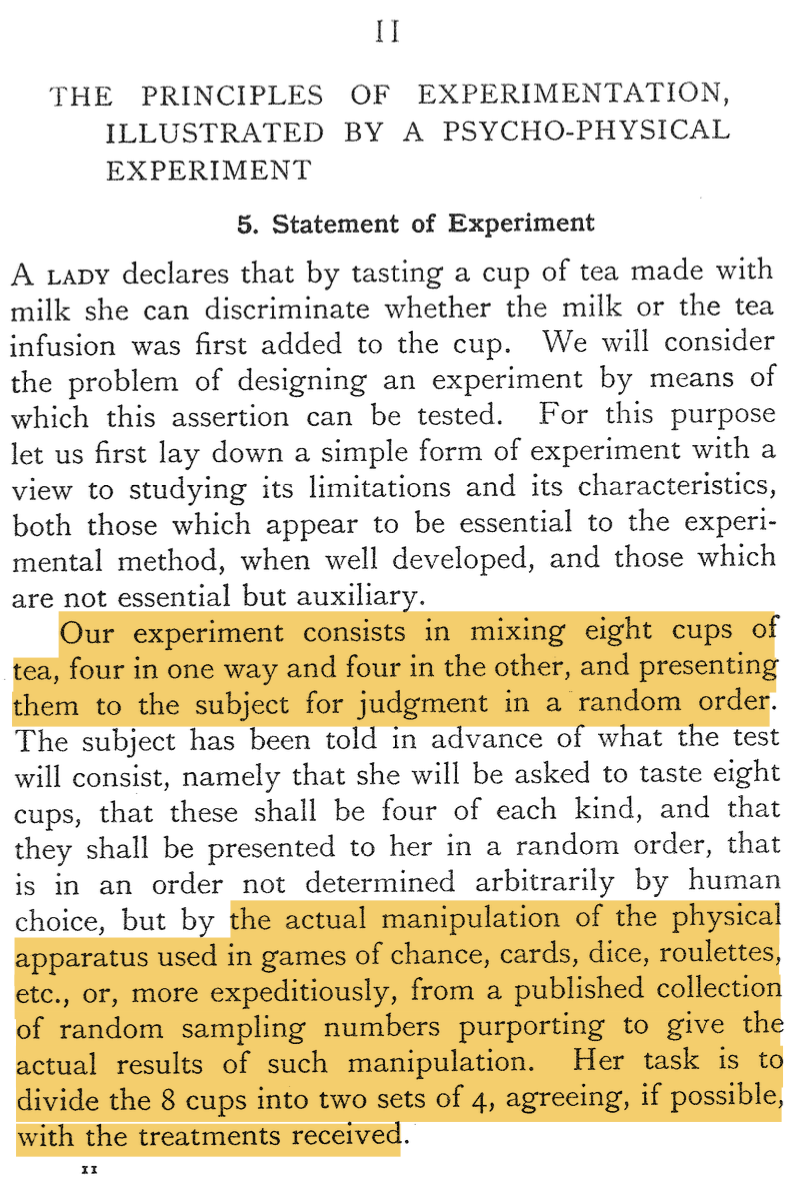
\includegraphics[width=0.5\linewidth]{images/fisher_lady_tasting_tea_text.png}
\end{figure} \vfill
\end{frame}
%---------------------------------------------------------------
\begin{frame}{Random assignment}
\vfill
\begin{itemize} \vfill
\item \textcolor{magenta}{Treatment Assignment} \vfill
\item[] Denote whether $i$th unit (cup) is assigned to treatment (milk-first) or control (tea-first) by $z_i = 1$ or $z_i = 0$ \vfill
\item[] Denote collection of all $N$ treatment indicator variables by \\ $\bm{z} = \begin{bmatrix} z_1 & z_2 & \ldots & z_N \end{bmatrix}^{\top}$ \vfill
\item[] There are $2^N$ ways one could assign $N$ units to treatment or control \vfill
\end{itemize} \vfill
\begin{equation}
\left\{0, 1\right\}^N = \left\{
\begin{bmatrix} 0 \\ 0 \\ 0 \\ 0 \\ 0 \\ 0 \\ 0 \\ 0 \end{bmatrix},
\begin{bmatrix} 1 \\ 0 \\ 0 \\ 0 \\ 0 \\ 0 \\ 0 \\ 0 \end{bmatrix},
\begin{bmatrix} 0 \\ 1 \\ 0 \\ 0 \\ 0 \\ 0 \\ 0 \\ 0 \end{bmatrix},
\cdots ,
\begin{bmatrix} 1 \\ 0 \\ 1 \\ 1 \\ 1 \\ 1 \\ 1 \\ 1 \end{bmatrix},
\begin{bmatrix} 0 \\ 1 \\ 1 \\ 1 \\ 1 \\ 1 \\ 1 \\ 1 \end{bmatrix},
\begin{bmatrix} 1 \\ 1 \\ 1 \\ 1 \\ 1 \\ 1 \\ 1 \\ 1 \end{bmatrix}
\right\}
\end{equation} \vfill
\end{frame}
%---------------------------------------------------------------
\begin{frame}{Random assignment}
\vfill
\begin{itemize} \vfill
\item For our purposes, a randomized design is a procedure for selecting any assignment from $\left\{0, 1\right\}^N$ with probability $p(\bm{z})$ \vfill
\item Therefore, $\bm{Z}$ is a random vector with support $\Omega \coloneqq \left\{\bm{z}: p(\bm{z}) > 0\right\}$ and $\Pr\left(\bm{Z} = \bm{z}\right) = p(\bm{z})$ \vfill
\item \textcolor{magenta}{Bernoulli (simple random) assignment} \vfill
\begin{itemize} \vfill
\item[] $N$ independent flips of (usually fair) coin \vfill
\end{itemize} \vfill
\item \textcolor{magenta}{Complete random assignment} \vfill
\begin{itemize} \vfill
\item[] $N$ draws from an urn in which some proportion are red (treated) balls and remaining proportion are blue (control) balls \vfill
\end{itemize} \vfill
\end{itemize} \vfill
\end{frame}
%---------------------------------------------------------------
\begin{frame}{Random assignment}
\vfill
\begin{itemize} \vfill
\item \citet[][p.~11]{fisher1935a}: \vfill
\begin{quote} \vfill
``Our experiment consists in mixing eight cups of tea, four in one way and four in the other, and presenting them to the subject for judgment in a random order.''
\end{quote} \vfill
\begin{itemize}
\item Support of $\bm{Z}$ is \vspace{-1.5em}
\begin{equation}
\left\{0, 1\right\}^N \supset \Omega = \left\{
\begin{bmatrix} 1 \\ 1 \\ 1 \\ 1 \\ 0 \\ 0 \\ 0 \\ 0 \end{bmatrix},
\begin{bmatrix} 1 \\ 1 \\ 1 \\ 0 \\ 1 \\ 0 \\ 0 \\ 0 \end{bmatrix},
\begin{bmatrix} 1 \\ 1 \\ 1 \\ 0 \\ 0 \\ 1 \\ 0 \\ 0 \end{bmatrix},
\cdots ,
\begin{bmatrix} 0 \\ 0 \\ 0 \\ 1 \\ 1 \\ 0 \\ 1 \\ 1 \end{bmatrix},
\begin{bmatrix} 0 \\ 0 \\ 0 \\ 1 \\ 0 \\ 1 \\ 1 \\ 1 \end{bmatrix},
\begin{bmatrix} 0 \\ 0 \\ 0 \\ 0 \\ 1 \\ 1 \\ 1 \\ 1 \end{bmatrix}
\right\}
\end{equation} \vspace{1em}
\item Probability of each assignment in $\Omega$ is $\Pr\left(\mathbf{Z} = \mathbf{z} \right) = \left\lvert \Omega \right\rvert^{-1}$ for all $\bm{z} \in \Omega$  \vfill
\item[] ($\left\lvert \Omega \right\rvert$ is the cardinality of, i.e., number of elements in, the set $\Omega$) \vfill
\end{itemize} \vfill
\end{itemize} \vfill
\end{frame}
%---------------------------------------------------------------
\begin{frame}{Randomization-based distributions}
\vfill
\begin{itemize}
\item Suppose first of $70$ assignments happened to be randomly selected \vfill 
\item The ``lady'' correctly identifies all $4$ milk-first and all $4$ tea-first cups \vfill
\vspace{1em}
\begin{table}[H]
\centering
\begin{tabular}{l|cc}
\toprule
Unit & $\bm{z}$ & $\bm{y}$ \\ 
  \midrule
$1$ & $1$ & $1$  \\ 
$2$ & $1$ & $1$  \\ 
$3$ & $1$ & $1$  \\ 
$4$ & $1$ & $1$  \\ 
$5$ & $0$ & $0$  \\ 
$6$ & $0$ & $0$  \\ 
$7$ & $0$ & $0$ \\ 
$8$ & $0$ & $0$ 
\end{tabular}
\caption{Results of R. A. Fisher's ``Lady Tasting Tea'' experiment}
\label{tab: lady tasting tea obs data}
\end{table}
\vspace{-2em}
\vfill
\item We summarize data by number of focal-group (milk-first) cups correctly identified, $\mathbf{z}^{\top}\mathbf{y}$, which in this case is $\mathbf{z}^{\top}\mathbf{y} = 4$ \vfill
\end{itemize} \vfill
\end{frame}
%---------------------------------------------------------------
\begin{frame}{Randomization-based distributions}
\vfill
\begin{itemize} \vfill
\item \citet{fisher1935a} entertained \textcolor{magenta}{counter-to-fact assignments of treatment}, holding responses fixed at their observed values \vfill
\item Responses fixed at observed values corresponds to scenario in which ``lady'' cannot discriminate between milk-first and tea-first cups \vfill
\end{itemize} \vfill 
\begin{table}[H]
\scriptsize
    \begin{tabular}{l|l}
    \toprule
    $\mathbf{z}_1$ & $\mathbf{y}$ \\ \midrule
    1 & 1  \\
    1 & 1   \\
    1 & 1   \\
    1 & 1  \\
    0 & 0  \\
    0 & 0  \\
    0 & 0  \\
    0 & 0  
    \end{tabular}
    \hfill
      \begin{tabular}{l|l}
      \toprule
    $\mathbf{z}_2$ & $\mathbf{y}$ \\ \midrule
    1 &  1  \\
    1 &  1  \\
    1 &  1  \\
    0 &  1   \\
    1 &  0  \\
    0 &  0  \\
    0 &  0  \\
    0 &  0  
    \end{tabular}
     \hfill
      \begin{tabular}{l|l}
      \toprule
    $\mathbf{z}_3$ & $\mathbf{y}$ \\ \midrule
    1 & 1  \\
    1 & 1  \\
    1 & 1  \\
    0 & 1   \\
    0 & 0  \\
    1 & 0  \\
    0 & 0  \\
    0 & 0  
    \end{tabular}
     \hfill
     $\cdots $
     \hfill
      \begin{tabular}{l|l}
      \toprule
    $\mathbf{z}_{68}$ & $\mathbf{y}$ \\ \midrule
    0 & 1  \\
    0 & 1  \\
    0 & 1  \\
    1 & 1   \\
    1 & 0  \\
    0 & 0  \\
    1 & 0  \\
    1 & 0  
    \end{tabular}
     \hfill
      \begin{tabular}{l|l}
      \toprule
    $\mathbf{z}_{69}$ & $\mathbf{y}$ \\ \midrule
    0 & 1  \\
    0 & 1  \\
    0 & 1  \\
    1 & 1  \\
    0 & 0 \\
    1 & 0  \\
    1 & 0  \\
    1 & 0  
    \end{tabular}
     \hfill
      \begin{tabular}{l|l}
      \toprule
    $\mathbf{z}_{70}$ & $\mathbf{y}$ \\ \midrule
    0 & 1  \\
    0 & 1  \\
    0 & 1  \\
    0 & 1  \\
    1 & 0   \\
    1 & 0  \\
    1 & 0  \\
    1 & 0  
    \end{tabular}
\label{tab: fisher's null pot outs schedule}
\end{table}
\end{frame}
%---------------------------------------------------------------
\begin{frame}{Randomization-based distributions}
\vfill
\begin{itemize} \vfill
\item \citet{fisher1935a} derived distribution of summary measure, $\bm{Z}^{\top} \bm{y}$, if ``lady'' could not discriminate between milk-first and tea-first cups \vfill
\end{itemize}  \vfill
\begin{figure}[H]
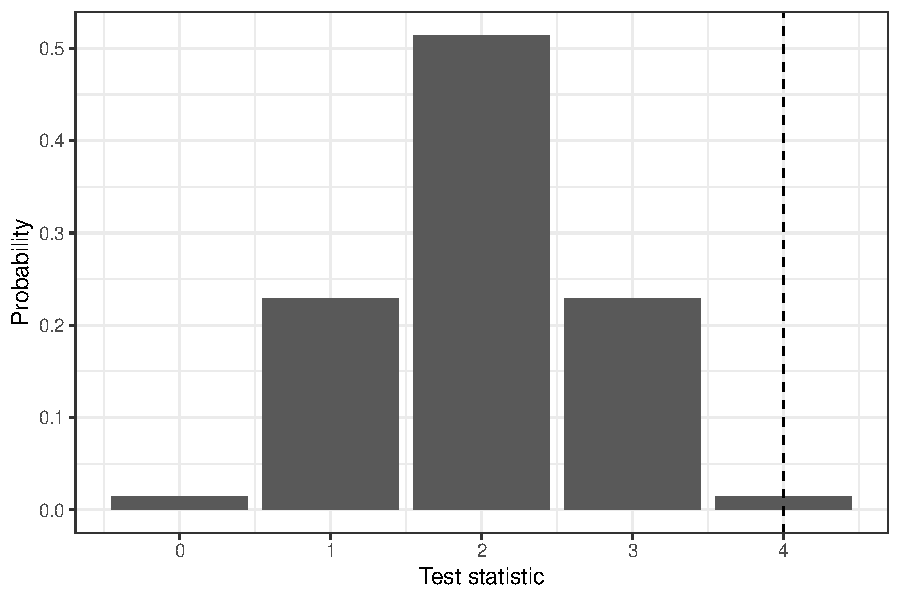
\includegraphics[width=0.9\linewidth]{null_dist_no_discrim_plot.pdf}
\end{figure} \vfill
\end{frame}
%---------------------------------------------------------------
\section{Potential Outcomes}
\begin{frame}{Potential outcomes}
\vfill
\begin{itemize} \vfill
\item Thus far, we have entertained counter-to-fact assignments of treatment \vfill
\begin{itemize} \vfill
\item[] Responses have been fixed at their observed values \vfill
\end{itemize} \vfill
\item \citet{neyman1923} and \citet{rubin1974} also posited counter-to-fact outcomes \vfill
\begin{itemize} \vfill
\item[] I.e., \textcolor{magenta}{potential outcomes} \vfill
\end{itemize} \vfill
\item E.g., perfect discrimination in ``Lady Tasting Tea'' example \vfill
\item[] \vfill
\vspace{2em}
\begin{table}[H]
\scriptsize
    \begin{tabular}{l|l}
    \toprule
    $\mathbf{z}_1$ & $\mathbf{y}$ \\ \midrule
    1 & 1  \\
    1 & 1   \\
    1 & 1   \\
    1 & 1  \\
    0 & 0  \\
    0 & 0  \\
    0 & 0  \\
    0 & 0  
    \end{tabular}
    \hfill
      \begin{tabular}{l|l}
      \toprule
    $\mathbf{z}_2$ & $\mathbf{y}$ \\ \midrule
    1 &  1  \\
    1 &  1  \\
    1 &  1  \\
    0 &  0   \\
    1 &  1  \\
    0 &  0  \\
    0 &  0  \\
    0 &  0  
    \end{tabular}
     \hfill
      \begin{tabular}{l|l}
      \toprule
    $\mathbf{z}_3$ & $\mathbf{y}$ \\ \midrule
    1 & 1  \\
    1 & 1  \\
    1 & 1  \\
    0 & 0   \\
    0 & 0  \\
    1 & 1  \\
    0 & 0  \\
    0 & 0  
    \end{tabular}
     \hfill
     $\cdots $
     \hfill
      \begin{tabular}{l|l}
      \toprule
    $\mathbf{z}_{68}$ & $\mathbf{y}$ \\ \midrule
    0 & 0  \\
    0 & 0  \\
    0 & 0  \\
    1 & 1   \\
    1 & 1  \\
    0 & 0  \\
    1 & 1  \\
    1 & 1  
    \end{tabular}
     \hfill
      \begin{tabular}{l|l}
      \toprule
    $\mathbf{z}_{69}$ & $\mathbf{y}$ \\ \midrule
    0 & 0  \\
    0 & 0  \\
    0 & 0  \\
    1 & 1  \\
    0 & 0 \\
    1 & 1  \\
    1 & 1  \\
    1 & 1  
    \end{tabular}
     \hfill
      \begin{tabular}{l|l}
      \toprule
    $\mathbf{z}_{70}$ & $\mathbf{y}$ \\ \midrule
    0 & 0  \\
    0 & 0  \\
    0 & 0  \\
    0 & 0  \\
    1 & 1   \\
    1 & 1  \\
    1 & 1  \\
    1 & 1  
    \end{tabular}
\end{table} \vfill
\end{itemize}  
\vfill
\end{frame}
%---------------------------------------------------------------
\begin{frame}{Potential outcomes}
\vfill
\begin{figure}[H]
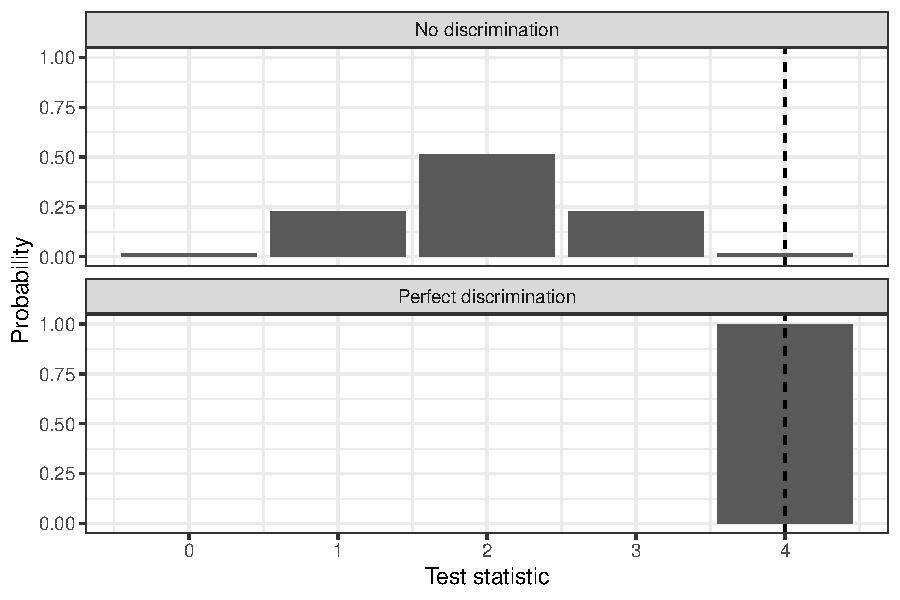
\includegraphics[width=1\linewidth]{null_dists_discrim_plot.pdf}
\end{figure} \vfill
\end{frame}
%---------------------------------------------------------------
\begin{frame}{Potential outcomes}
\vfill
\begin{itemize} \vfill
\item A \mh{potential outcome schedule} is vector-valued function $\bm{y}: \left\{0, 1\right\}^N \mapsto \R^N$ \vfill
\begin{itemize} \vfill
\item Potential outcomes for all $N$ units written as $\bm{y}(\bm{z})$ \vfill
\item Potential outcome for individual unit $i$ written as $y_i(\bm{z})$ \vfill
\end{itemize} \vfill
\item Intuitively, a listing of how each unit would respond to any $\bm{z} \in \left\{0, 1\right\}^N$ \vfill
\item We often consider potential outcome schedules that satisfy Stable Unit Treatment Value Assumption (SUTVA) \citep{cox1958a,rubin1980b,rubin1986} \vfill
\item SUTVA means that \vfill
\begin{enumerate} \vfill
\item Units in experiment respond to only treatment condition to which each unit is individually assigned \vfill
\item Treatment condition is actually the same treatment for all units assigned to treatment and control condition is the same for all units assigned to control \vfill
\end{enumerate} \vfill
\end{itemize}  
\vfill
\end{frame}
%---------------------------------------------------------------
\begin{frame}{Potential outcomes}
\vfill
\begin{itemize} \vfill
\item SUTVA implies \vfill
\begin{itemize} \vfill
\item One fixed value of the outcome for unit $i$ if it is assigned to treatment $(z_i = 1)$ and another fixed value if unit $i$ is assigned to control $(z_i = 0)$ \vfill
\item[] $\rightarrow$ write potential outcomes for unit $i$ as $y_i(1)$ or $y_i(0)$ \vfill 
\item Each unit has at most two potential outcomes \vfill
\end{itemize} \vfill 
\end{itemize} 
\vfill
\end{frame}
%---------------------------------------------------------------
\begin{frame}{Potential outcomes}
\vfill
\begin{itemize} \vfill
\item Both no discrimination and perfect discrimination satisfy SUTVA \vfill
\vspace{0.5em}
\item Consider, e.g., unit $i = 4$ under each potential outcome schedule \vfill
\begin{itemize} \vfill
\vspace{1em}
\item \textbf{No discrimination} \vfill
\vspace{1em}
\begin{table}[H]
\scriptsize
    \begin{tabular}{l|l}
    $\mathbf{z}_1$ & $\mathbf{y}$ \\ \midrule
    1 & 1  \\
    1 & 1   \\
    1 & 1   \\
    \mh{1} & \mh{1}  \\
    0 & 0  \\
    0 & 0  \\
    0 & 0  \\
    0 & 0  
    \end{tabular}
    \hfill
      \begin{tabular}{l|l}
    $\mathbf{z}_2$ & $\mathbf{y}$ \\ \midrule
    1 &  1  \\
    1 &  1  \\
    1 &  1  \\
    \mh{0} &  \mh{1}   \\
    1 &  0  \\
    0 &  0  \\
    0 &  0  \\
    0 &  0  
    \end{tabular}
     \hfill
      \begin{tabular}{l|l}
    $\mathbf{z}_3$ & $\mathbf{y}$ \\ \midrule
    1 & 1  \\
    1 & 1  \\
    1 & 1  \\
    \mh{0} & \mh{1}   \\
    0 & 0  \\
    1 & 0  \\
    0 & 0  \\
    0 & 0  
    \end{tabular}
     \hfill
     $\cdots $
     \hfill
      \begin{tabular}{l|l}
    $\mathbf{z}_{68}$ & $\mathbf{y}$ \\ \midrule
    0 & 1  \\
    0 & 1  \\
    0 & 1  \\
    \mh{1} & \mh{1}   \\
    1 & 0  \\
    0 & 0  \\
    1 & 0  \\
    1 & 0  
    \end{tabular}
     \hfill
      \begin{tabular}{l|l}
    $\mathbf{z}_{69}$ & $\mathbf{y}$ \\ \midrule
    0 & 1  \\
    0 & 1  \\
    0 & 1  \\
    \mh{1} & \mh{1}  \\
    0 & 0 \\
    1 & 0  \\
    1 & 0  \\
    1 & 0  
    \end{tabular}
     \hfill
      \begin{tabular}{l|l}
    $\mathbf{z}_{70}$ & $\mathbf{y}$ \\ \midrule
    0 & 1  \\
    0 & 1  \\
    0 & 1  \\
    \mh{0} & \mh{1}  \\
    1 & 0   \\
    1 & 0  \\
    1 & 0  \\
    1 & 0  
    \end{tabular}
\end{table} \vfill
\vspace{1em}
\item \textbf{Perfect discrimination} \vfill
\vspace{1em}
\begin{table}[H]
\scriptsize
    \begin{tabular}{l|l}
    $\mathbf{z}_1$ & $\mathbf{y}$ \\ \midrule
    1 & 1  \\
    1 & 1   \\
    1 & 1   \\
    \mh{1} & \mh{1}  \\
    0 & 0  \\
    0 & 0  \\
    0 & 0  \\
    0 & 0  
    \end{tabular}
    \hfill
      \begin{tabular}{l|l}
    $\mathbf{z}_2$ & $\mathbf{y}$ \\ \midrule
    1 &  1  \\
    1 &  1  \\
    1 &  1  \\
    \mh{0} &  \mh{0}   \\
    1 &  1  \\
    0 &  0  \\
    0 &  0  \\
    0 &  0  
    \end{tabular}
     \hfill
      \begin{tabular}{l|l}
    $\mathbf{z}_3$ & $\mathbf{y}$ \\ \midrule
    1 & 1  \\
    1 & 1  \\
    1 & 1  \\
    \mh{0} & \mh{0}   \\
    0 & 0  \\
    1 & 1  \\
    0 & 0  \\
    0 & 0  
    \end{tabular}
     \hfill
     $\cdots $
     \hfill
      \begin{tabular}{l|l}
    $\mathbf{z}_{68}$ & $\mathbf{y}$ \\ \midrule
    0 & 0  \\
    0 & 0  \\
    0 & 0  \\
    \mh{1} & \mh{1}   \\
    1 & 1  \\
    0 & 0  \\
    1 & 1  \\
    1 & 1  
    \end{tabular}
     \hfill
      \begin{tabular}{l|l}
    $\mathbf{z}_{69}$ & $\mathbf{y}$ \\ \midrule
    0 & 0  \\
    0 & 0  \\
    0 & 0  \\
    \mh{1} & \mh{1}  \\
    0 & 0 \\
    1 & 1  \\
    1 & 1  \\
    1 & 1  
    \end{tabular}
     \hfill
      \begin{tabular}{l|l}
    $\mathbf{z}_{70}$ & $\mathbf{y}$ \\ \midrule
    0 & 0  \\
    0 & 0  \\
    0 & 0  \\
    \mh{0} & \mh{0}  \\
    1 & 1   \\
    1 & 1  \\
    1 & 1  \\
    1 & 1  
    \end{tabular}
\end{table} \vfill
\end{itemize}  \vfill
\end{itemize}\vfill
\end{frame}
%---------------------------------------------------------------
\begin{frame}{Potential outcomes}
\vfill
\begin{itemize} \vfill
\item \mh{Fundamental Problem of Causal Inference} \citep{holland1986} \vfill
  \begin{center}
    We can never observe both $y_{i}(1)$ and $y_{i}(0)$ for the same $i$\\
  \end{center} \vfill
\item We can observe only one of the two potential outcomes
  $$ y_i = z_i y_{i}(1) + (1 - z_i)y_{i}(0)$$ \vfill 
\item Analogue without supposing SUTVA \vfill
\begin{itemize} \vfill
\item We can observe $y_i(\bm{z})$ under only one $\bm{z} \in \left\{0, 1\right\}^N$ \vfill
\end{itemize} \vfill
\end{itemize}  
\vfill
\end{frame}
%---------------------------------------------------------------
\section{Next class: Hypothesis testing}
\begin{frame}{Hypothesis testing}
\vfill
\begin{itemize} \vfill
\item Use known assignment mechanism to \textcolor{magenta}{reliably} gather evidence \vfill
\begin{itemize} \vfill
\item against null hypothesis about one potential outcome schedule \\ (e.g., no discrimination) \vfill
\item and in favor of alternative hypothesis about another \\ (e.g., perfect discrimination) \vfill
\end{itemize} \vfill
\end{itemize} \vfill
\end{frame}
%---------------------------------------------------------------

\begin{frame}
\frametitle{References} 
\scriptsize
\bibliographystyle{chicago}
\bibliography{Master_Bibliography}   % name your BibTeX data base
\end{frame}
%---------------------------------------------------------------
\end{document}